%% -*- mode: latex; mode: reftex; mode: flyspell; TeX-master: "top.tex"; -*-


The  process  of forming  functional  connections  between neurons  is
complex  and   dynamic.   Time-lapse  microscopy   has  revealed  that
differentiating  neurons undergo  a large  range of  dynamic processes
including cell body motility, filopodial dynamics, and repeated cycles
of  neurite growth  and  retraction.  Of  critical  importance is  the
process  by which  axons and  dendrites are  formed in  which a neurite
ceases retracting, extends a   long  distance, and  forms
a connection. Such  dynamic events are  governed by a  complex protein
network that  coordinates   dynamic functions 
within the cytoskeleton, membrane, etc.

Powerful tools such as 
RNA interference  (RNAi)
technology,  fluorescent  protein   labeling,  image  processing,  and
automated high-throughput  microscopy have  opened the door  for large
scale  perturbation studies to help investigate such processes. RNAi  screens have  already led  to novel
insights   into  a  number   of  cellular   processes  such   as  cell
migration~\cite{Bakal07}  and endocytosis~\cite{Collinet10}.  However,
limitations  in  image  processing  have  restricted  most
investigations to static image analysis.

Knowledge  of dynamics is  essential if we are  to understand
complex  processes such  as neuron  morphogenesis.  However, designing
algorithms to quantify dynamic  behaviors is challenging, and
automatic methods  have appeared only  very recently. State-of-the-art
high-throughput techniques have successfully quantified morphodynamics
of  HeLA cancer  cells  in an  effort  to understand 
mitosis~\cite{Held10,Neumann10,Zhu05}.   However,  the morphology  and
dynamics of  cells in previous studies are simple compared to neurons,
whose highly deformable  neurites that branch, expand,
retract, and collapse. 

%% gg 20121023 - modified greedy, added time-lapse sequence
In this paper, we propose a  fully automatic method for detecting, tracking, and
segmenting {\em  every component  of the neuron}  (nucleus, soma,  neurites, and
filopodia), and quantifying their dynamic behaviors in ways that were previously
not possible. Our  approach begins with a tracking step that detects nuclei at each  time step and
associates nuclei  belonging to the  same neuron  throughout the
time-lapse sequence.
Using tracked nuclei as  seed points, a region-growing  algorithm segments
the neuron's soma.  The somata are  used to initialize a  joint segmentation of
the entire structure  of all neurons in a  image using a probabilistic
method based on  shortest path computations.  A graph  describing the morphology
of  the neurites  is extracted  from this  segmentation.  Each  neurite  tree is
tracked by association, and filopodia  are detected by analyzing the topology of
the tracked  neurites.  Finally,  a set of  156 {\em morphodynamic  features} is
extracted, quantifying the behavior of the each neuron in the video.


As   demonstrated  in   Fig.~\ref{fig:video}, 
our  approach produces reliable  segmentations capable of capturing
complex  neuron  dynamics. To validate our approach, we analyzed a   
small-scale  siRNA screen  of 5  genes (3  siRNAs/gene). Our analysis
confirmed steady-state phenotypes obtained previously using 
MetaMorph\texttrademark~\cite{Pertz08}. We were also able to
quantify dynamic behaviors which had been previously observed, but never
measured~\cite{Pertz08}. Our  analysis also uncovered
new dynamic behaviors which are only apparant through dynamic analysis.

%While  our greedy tracking  and probabilistic  segmentation algorithms are  novel,  they are designed to be efficient and thus are relatively simple.  The  main contribution of this  paper is the  system as a whole,  which  is capable  of  high-throughput  processing of  videos, tracking individual  parts of  neurons, and quantifying  their dynamic behaviors in ways that were previously not possible.





%39ba1a
%----------------------------------------------------------------------------
\begin{figure*}[t]
       \begin{tabular}{@{\hspace{0mm}}c@{}|@{}c@{}|@{}c@{}}
        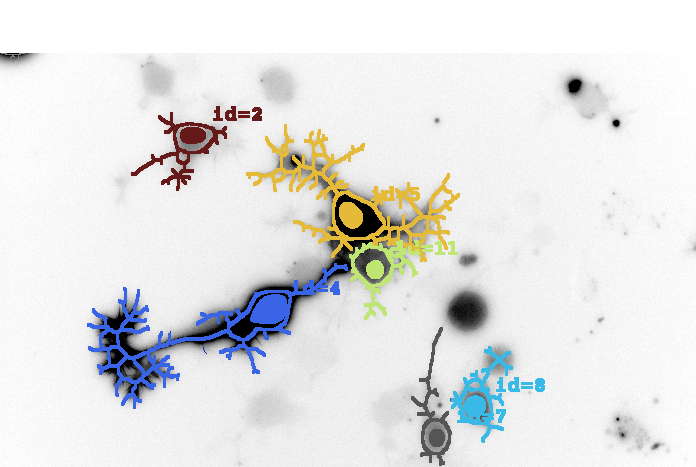
\includegraphics[width=60mm] {images/mv1_008_crop.png} &
        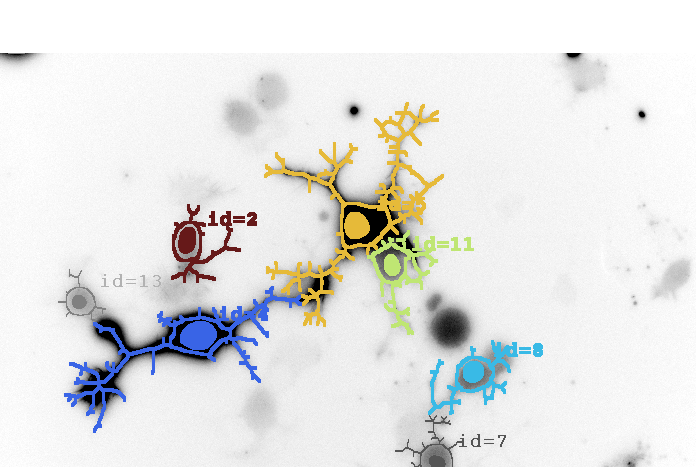
\includegraphics[width=60mm] {images/mv1_017_crop.png}  &
        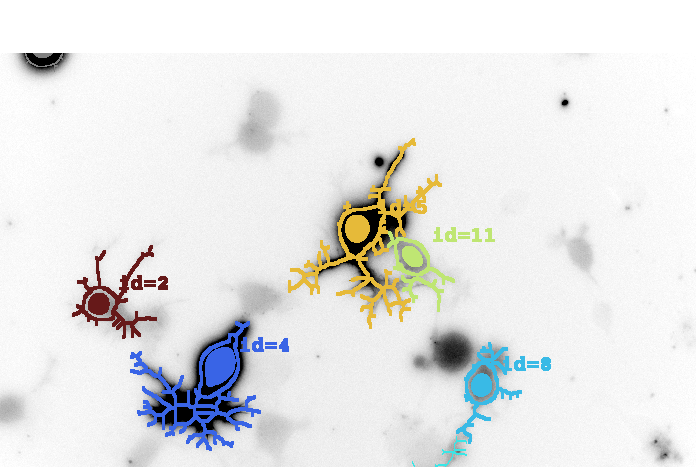
\includegraphics[width=60mm] {images/mv1_026_crop.png} \\ [-.8ex]
        \hline \\ [-2.9ex]
       \end{tabular} 
      \begin{tabular}{@{\hspace{0mm}}c@{}c@{}|@{}c@{}c@{}|@{}c@{}c@{}}
        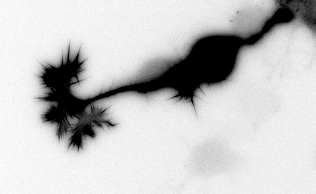
\includegraphics[width=30mm] {images/0_008.png} & 
        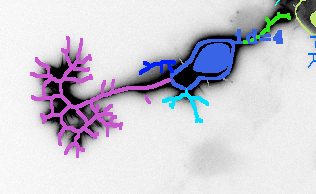
\includegraphics[width=30mm] {images/2_008_thick.png} & 
        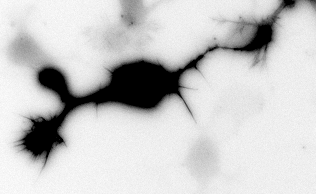
\includegraphics[width=30mm] {images/0_017.png} & 
	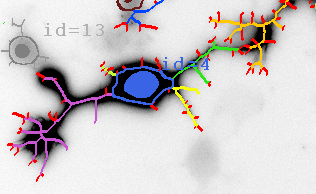
\includegraphics[width=30mm] {images/2_017_thick.png} & 
        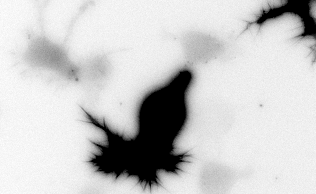
\includegraphics[width=30mm] {images/0_026.png} &
        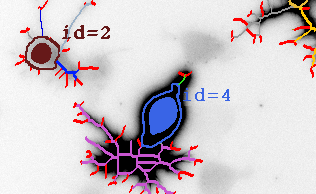
\includegraphics[width=30mm] {images/2_026_thick.png} \\ [-1ex]
	\multicolumn{2}{c}{\footnotesize $t = 80$ min} & 
	\multicolumn{2}{c}{\footnotesize $t = 170$ min} & 
	\multicolumn{2}{c}{\footnotesize $t = 260$ min} \\
      \end{tabular} 
    \vspace{-2mm}  
    \caption{\footnotesize Our approach tracks and segments the entire neuron. The top
        row contains our results from an experiment where 
	MAP2K7 gene functions are inhibited.  Image contrast has been 
	enhanced for visibility.  Tracked neurons are marked by a unique color and id.   
	Nuclei  are denoted  by  filled  ellipsoids, somata  as
        contours,  and neurites  as trees.   The bottom shows details
        from  above: {\it (left)}  original  image {\it (right)}  individual neurites
        marked with a different colors. Our  approach   performs  well  even  in  challenging
        situations where neurons appear in close proximity. Note: faintly  stained
        cells are ignored for robustness.}
    \label{fig:video}
\vspace{-4mm}
\end{figure*}
%----------------------------------------------------------------------------



%%----------------------------------------------------------------------------
%\begin{figure}[t]
%       \begin{tabular}{@{\hspace{0mm}}c@{}|@{}c@{}}
%        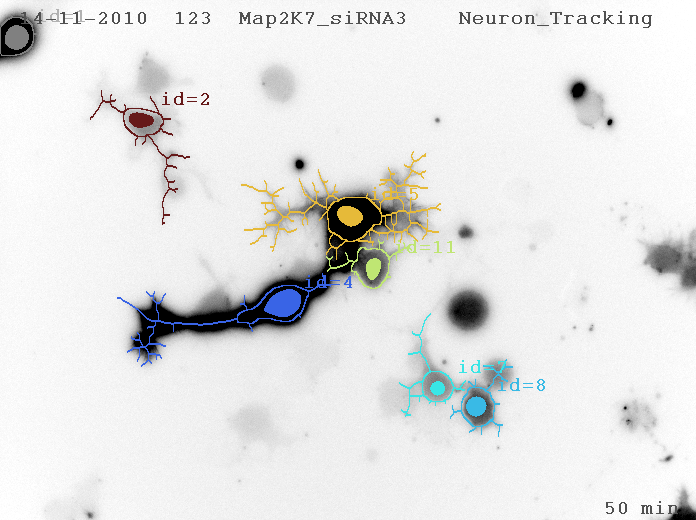
\includegraphics[width=45mm] {images/mv1_005.png}  &
%        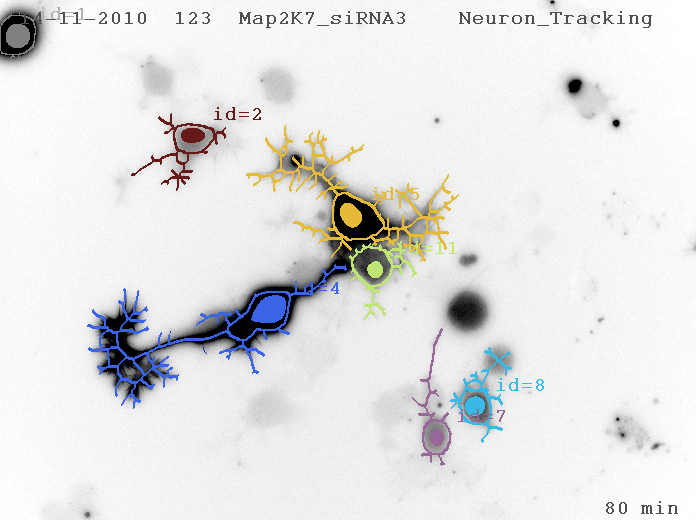
\includegraphics[width=45mm] {images/mv1_008.png} \\ [-.8ex]
%        \hline \\ [-2.6ex]
%        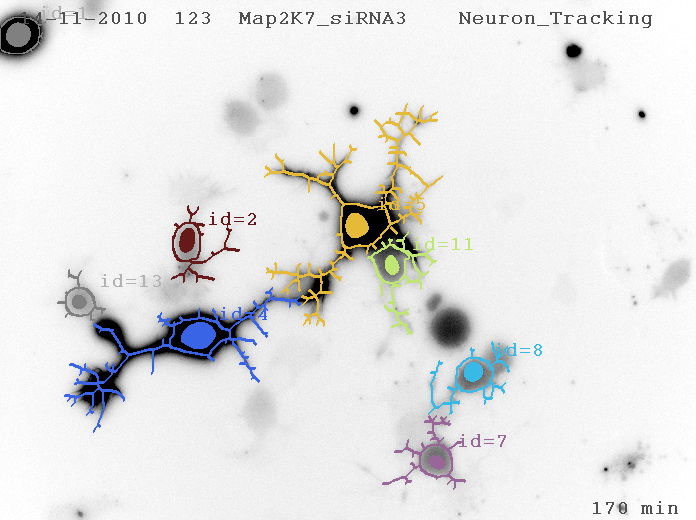
\includegraphics[width=45mm] {images/mv1_017.png}  &
%        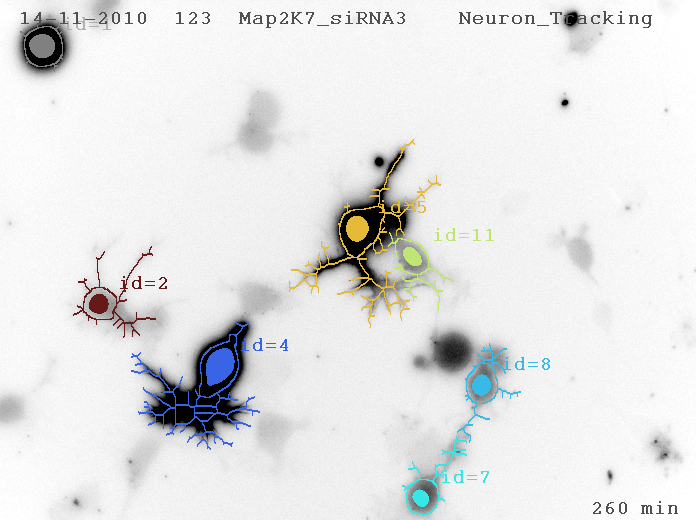
\includegraphics[width=45mm] {images/mv1_026.png} \\ [-.8ex]
%        \hline \\ [-2.9ex]
%       \end{tabular} 
%       
%      \begin{tabular}{@{\hspace{0mm}}c@{}c@{}c@{}c@{}}
%        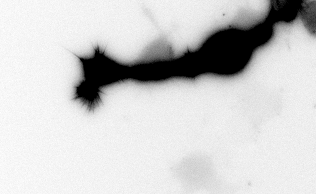
\includegraphics[width=22.5mm] {images/0_005.png} &
%        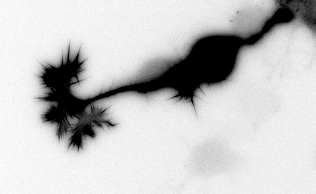
\includegraphics[width=22.5mm] {images/0_008.png} & 
%        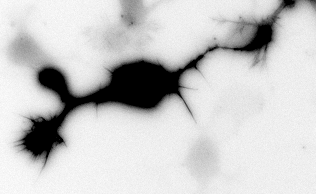
\includegraphics[width=22.5mm] {images/0_017.png} & 
%        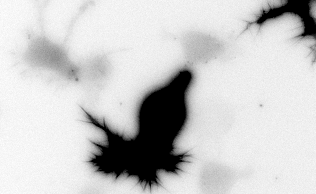
\includegraphics[width=22.5mm] {images/0_026.png} \\ [-1ex]
%        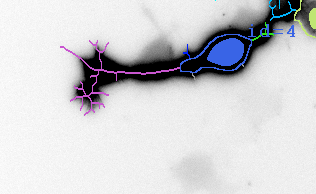
\includegraphics[width=22.5mm] {images/2_005.png} &
%        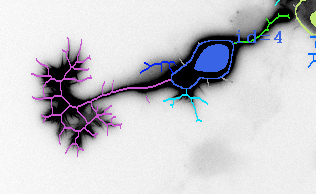
\includegraphics[width=22.5mm] {images/2_008.png} & 
%        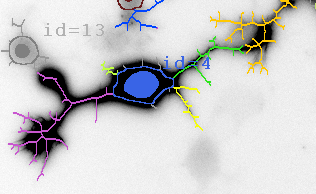
\includegraphics[width=22.5mm] {images/2_017.png} & 
%        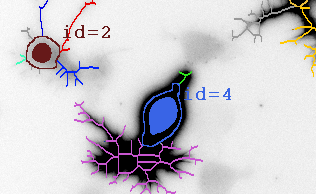
\includegraphics[width=22.5mm] {images/2_026.png} \\ [-1ex]
%        %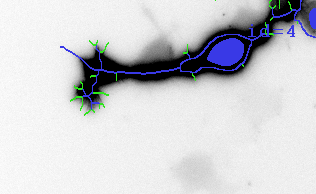
\includegraphics[width=22.5mm] {images/3_005.png} &
%        %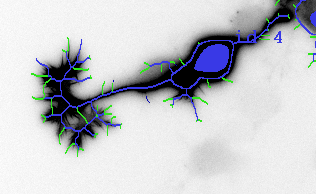
\includegraphics[width=22.5mm] {images/3_008.png} & 
%        %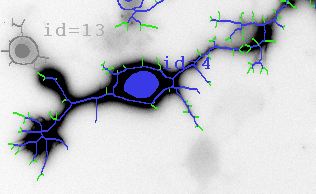
\includegraphics[width=22.5mm] {images/3_017.png} & 
%        %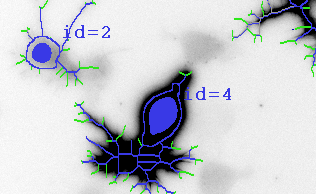
\includegraphics[width=22.5mm] {images/3_026.png} \\ [-1ex]
%        {\footnotesize $t = 50$ min} & 
%        {\footnotesize $t = 80$ min} & 
%        {\footnotesize $t = 170$ min} & 
%        {\footnotesize $t = 260$ min} \\ [-1ex]
%      \end{tabular}
%    \vspace{-2mm}  
%    \caption{ {\footnotesize {\it Neuron  Tracking Results.  } The top
%        two rows  contain frames from an experiment  where MAP2K7 gene
%        functions are inhibited.  For visibility we enhanced the image
%        contrast.  Tracked neurons are marked by a unique color and id
%        tag.   Nuclei  are denoted  by  filled  ellipsoids, somata  as
%        contours,  and neurites  as trees.   Bottom rows  show details
%        from  above: 1)  enhanced original  image 2)  tracked neurites
%        marked with a different colors. Our  approach   performs  well  even  in  challenging
%        situations where neurons appear in close proximity. Note: faintly  stained
%        cells are ignored for robustness.}}
%    \label{fig:video}
%\vspace{-6mm}
%\end{figure}
%%----------------------------------------------------------------------------


